\documentclass[a4paper,10pt]{article}
\usepackage[utf8]{inputenc}
\usepackage[T1]{fontenc}
\usepackage[margin=0.75in]{geometry}
\usepackage{paralist}
\usepackage{fancyhdr}
\usepackage{listings}
\usepackage[colorlinks]{hyperref}
\usepackage{amssymb}
\usepackage{amsmath}
\usepackage{tcolorbox}
\usepackage{booktabs}
\usepackage{wrapfig}
\usepackage{xspace}
% Alwayws load this last
\usepackage{xcolor}
\usepackage{soul}

\def\chpcolor{blue!60}
\def\chpcolortxt{blue!60}
\def\sectionfont{\sffamily\Large}

\setcounter{secnumdepth}{2}

\makeatletter
%Section:
\def\@sectionstrut{\vrule\@width\z@\@height12.5\p@}
\def\@makesectionhead#1{%
  {\par\vspace{20pt}%
   \parindent 0pt\raggedleft\sectionfont
   \colorbox{\chpcolor}{%
     \parbox[t]{25pt}{\color{white}\@sectionstrut\@depth4.5\p@\hfill
       \ifnum\c@secnumdepth>\z@\thesection\fi}%
   }%
   \begin{minipage}[t]{\dimexpr\textwidth-25pt-2\fboxsep\relax}
   \color{\chpcolortxt}\@sectionstrut\hspace{5pt}#1
   \end{minipage}\par
   \vspace{10pt}%
  }
}
\def\section{\@afterindentfalse\secdef\@section\@ssection}
\def\@section[#1]#2{%
  \ifnum\c@secnumdepth>\m@ne
    \refstepcounter{section}%
    \addcontentsline{toc}{section}{\protect\numberline{\thesection}\textbf{#1}}%
  \else
    \phantomsection
    \addcontentsline{toc}{section}{#1}%
  \fi
  \sectionmark{\textbf{#1}}%
  \if@twocolumn
    \@topnewpage[\@makesectionhead{#2}]%
  \else
    \@makesectionhead{\textbf{#2}}\@afterheading
  \fi
}
\def\@ssection#1{%
  \if@twocolumn
    \@topnewpage[\@makesectionhead{#1}]%
  \else
    \@makesectionhead{#1}\@afterheading
  \fi
}
\makeatother




\makeatletter
\def\@makesubsectionhead#1{%
  {\par\vspace{20pt}%
   \parindent 0pt\raggedleft\sffamily\large
   \ifnum\c@secnumdepth>\z@\color{\chpcolortxt}{\thesubsection}\fi%
   %
   \begin{minipage}[t]{\dimexpr\textwidth-2\fboxsep\relax}
   \vspace{-10pt}\color{black}\hspace{5pt}#1
   \end{minipage}\\[-10pt]
   \noindent\rule{\textwidth}{1pt}\par
   \vspace{10pt}%
  }
}
\def\subsection{\@afterindentfalse\secdef\@subsection\@ssection}
\def\@subsection[#1]#2{%
  \ifnum\c@secnumdepth>\m@ne
    \refstepcounter{subsection}%
    \addcontentsline{toc}{subsection}{\protect\numberline{\thesubsection}\textbf{#1}}%
  \else
    \phantomsection
    \addcontentsline{toc}{subsection}{\textbf{#1}}%
  \fi
  \sectionmark{\textbf{#1}}%
  \if@twocolumn
    \@topnewpage[\@makesubsectionhead{\textbf{#2}}]%
  \else
    \@makesubsectionhead{\textbf{#2}}\@afterheading
  \fi
}
\def\@ssection#1{%
  \if@twocolumn
    \@topnewpage[\@makesubsectionhead{\textbf{#1}}]%
  \else
    \@makesubsectionhead{\textbf{#1}}\@afterheading
  \fi
}
\makeatother



\definecolor{codegreen}{rgb}{0,0.6,0}
\definecolor{codegray}{rgb}{0.5,0.5,0.5}
\definecolor{codepurple}{rgb}{0.58,0,0.82}
\definecolor{backcolour}{rgb}{0.95,0.95,0.92}

%Code listing style named "mystyle"
\lstdefinestyle{mystyle}{
  backgroundcolor=\color{backcolour},   commentstyle=\color{codegreen},
  keywordstyle=\color{magenta},
  numberstyle=\tiny\color{codegray},
  stringstyle=\color{codepurple},
  basicstyle=\ttfamily\footnotesize,
  breakatwhitespace=false,         
  breaklines=true,                 
  captionpos=b,                    
  keepspaces=true,                 
  numbers=left,                    
  numbersep=5pt,                  
  showspaces=false,                
  showstringspaces=false,
  showtabs=true,                  
  tabsize=2
}

%"mystyle" code listing set
\lstset{style=mystyle}


\newcommand{\xhdr}[1]{\vspace{10pt}\noindent{\color{blue!60}\textbf{#1}}}


\newcommand{\task}[1]{ {\color{blue!60}\noindent $\mathbf{\blacktriangleright}$ \texttt{#1}}}


\usepackage{tcolorbox}
\newtcolorbox{taskbox}{
    arc=0pt,
    boxrule=1pt,
    colback=gray!10,
    colframe=blue!60,
    width=\textwidth,
    halign=left,
}
\usepackage{tikz}
\usetikzlibrary{automata, positioning, arrows}
\usepackage{multicol}

\setlength{\parskip}{3pt}


\newcommand{\xb}{\mathbf{x}}
\newcommand{\wb}{\mathbf{w}}

\begin{document}
\tikzset{
->, % makes the edges directed
>=stealth, % makes the arrow heads bold
node distance=2cm, % specifies the minimum distance between two nodes. Change if necessary.
every state/.style={thick, fill=gray!10}, % sets the properties for each ’state’ node
initial text=$ $, % sets the text that appears on the start arrow
}

\sffamily

\newcommand{\nb}{Na\"ive Bayes\xspace}

\begin{center}
\noindent\rule{\textwidth}{1pt}\\[10pt]
{\color{blue!60}{CS434 Machine Learning and Data Mining -- Homework 3}}\\[10pt]
{\LARGE \nb and Neural Networks }\\[10pt]

\noindent\rule{\textwidth}{1pt}
\end{center}

\noindent\textbf{Overview and Objectives.} In this homework, we are going to do some exercises to understand \nb a bit better and then get some hand-on experience with simple Neural Networks in a multi-class classification setting.\\

\noindent\textbf{How to Do This Assignment.}
\begin{itemize}
    \item Each question that you need to respond to is in a blue "Task Box" with its corresponding point-value listed. 
    \item We prefer typeset solutions (\LaTeX~/ Word) but will accept scanned written work if it is legible. If a TA can't read your work, they can't give you credit. 
    \item Programming should be done in Python and numpy. If you don't have Python installed, you can install it from \href{https://www.python.org/downloads/}{here}. This is also the link showing \href{https://numpy.org/install/}{how to install numpy}. You can also search through the internet for numpy tutorials if you haven't used it before. Google and APIs are your friends!
\end{itemize}

\noindent\textbf{You are {\color{red}NOT} allowed to...}
\begin{itemize}
    \item Use machine learning package such as \lstinline{sklearn}. 
    \item Use data analysis package such as \lstinline{panda} or \lstinline{seaborn}.
    \item Discuss low-level details or share code / solutions with other students.
\end{itemize}

\noindent\textbf{Advice.} Start early. There are two sections to this assignment -- one involving working with math (20\% of grade) and another focused more on programming (80\% of the grade). Read the whole document before deciding where to start. 

\noindent\textbf{How to submit.} Submit a zip file to Canvas. Inside, you will need to have all your working code and \lstinline{hw3-report.pdf}. You will also submit test set predictions to a \href{https://www.kaggle.com/t/c4de5ee4c2ef45858c15e3183d24b2c0}{class-wide Kaggle competition}. 

\vspace{-10pt}
\section{Written Exercises: Analyzing \nb [5pts]}

\vspace{-20pt}
\subsection{Bernoulli Na\"ive Bayes As A Linear Classifier}
Consider a \nb model for binary classification where the features $X_1, ..., X_d$ are also binary variables. As part of training this \nb model, we would estimate the conditional distributions $P(X_i | y{=}c)$ for $c=\{0,1\}$ and $i=1,...,d$ as well as the prior distribution $P(y{=}c)$ for $c=\{0,1\}$. For notational simplicity, let's denote $P(X_i{=}1 | y{=}c)$ as $\theta_{ic}$ and $P(X_i{=}0 | y{=}c)$ as $1-\theta_{ic}$. Likewise, let $\theta_1$ be $P(y{=}1)$ and $\theta_0 = 1-\theta_1$ be $P(y{=}0)$. \\

\noindent If we write out the posterior of this classifier (leaving out the normalizing constant), we would have:
%
\begin{eqnarray}
    P(y=1 | x_1,...,x_d) ~=~ \frac{P(y=1) \prod_{i=1}^d P(x_i | y=1)}{P(x_1, ..., x_d)} ~\propto~ \theta_1 \prod_{i=1}^d \theta_{i1}^{x_i} (1-\theta_{i1})^{1-x_i}\label{eq:post1}\\[5pt]
    P(y=0 | x_1,...,x_d) ~=~ \frac{P(y=0)\prod_{i=1}^dP(x_i | y=0)}{P(x_1, ..., x_d)} ~\propto~ \theta_0 \prod_{i=1}^d \theta_{i0}^{x_i} (1-\theta_{i0})^{1-x_i}
    \label{eq:post2}
\end{eqnarray}
%
\noindent The classification rule in \nb is to choose the class with the highest posterior probability, that is to say by predicting $y = \mbox{argmax}_{c}~~P(y=c|x_1,...,x_d)$ for a new example $\mathbf{x} = [x_1, ..., x_d]$. In order for the prediction to be class 1, $P(y=1 | x_1,...,x_d)$ must be greater than $P(y=0 | x_1,...,x_d)$, or equivalently we could check if:
%
\begin{equation}
    \frac{P(y=1 | x_1,...,x_d)}{P(y=0 | x_1,...,x_d)} > 1
    \label{eq:logratio}
\end{equation}
%
\noindent In this setting with binary inputs, we will show that this is a linear decision boundary. This also true for continuous inputs if they are modelled with a member of the exponential family (including Gaussian) -- see \href{https://www.cs.cmu.edu/~tom/mlbook/NBayesLogReg.pdf}{proof here in \S 3.1}. 


\begin{taskbox}
\task{Q1 Prove Bernoulli \nb has a linear decision boundary [4pts].} Prove the Bernoulli \nb model described above has a linear decision boundary. Specifically, you'll need to show that class 1 will be predicted only if $b+\mathbf{w}^T\mathbf{x} > 0$ for some parameters $b$ and $\mathbf{w}$. To do so, show that:
%
\begin{equation}
    \frac{P(y=1 | x_1,...,x_d)}{P(y=0 | x_1,...,x_d)} > 1 ~~\Longrightarrow~~ b+\sum_{i=1}^d w_ix_i > 0
\end{equation}
%
As part of your report, explicitly write expressions for the bias $b$ and each weight $w_i$.\\[5pt]

\emph{\textbf{Hints:}} Expand Eq.~\eqref{eq:logratio} by substituting the posterior expressions from Eq.~\eqref{eq:post1} \& \eqref{eq:post2} into Eq.~\eqref{eq:logratio}. Take the log of that expression and combine like-terms. 
\end{taskbox}


\subsection{Duplicated Features in \nb}
\nb classifiers assume features are conditionally independent given the class label. When this assumption is violated, \nb classifiers may be over-confident or under-confident in the outputs. To examine this more closely, we'll consider the situation where an input feature is duplicated. These duplicated features are maximally dependent -- making this is a strong violation of conditional independence. Here, we'll examine a case where the confidence increases when the duplicated features are included \emph{despite no new information actually being added as input.}

\begin{taskbox}
\task{Q2 Duplicate Features in \nb [1pts].} Consider a \nb model with a single feature $X_1$ for a binary classification problem. Assume a uniform prior such that $P(y=0) = P(y=1)$. Suppose the model predicts class 1 for an example $\mathbf{x}$ then we know:
%
\begin{equation}
    P(y=1|X_1=x_1) > P(y=0|X_1=x_1)
    \label{eq:ineq}
\end{equation}
%
Now suppose we make a mistake and duplicate the $X_1$ feature in our data -- now we have two identical inputs $X_1$ and $X_2$. Show that the predicted probability for class 1 is higher than it was before; that is, prove:

\begin{equation}
    P(y=1|X_1=x_1, X_2=x_2) > P(y=1|X_1=x_1)
    \label{eq:prove}
\end{equation}\\[5pt]

\emph{\textbf{Hints:}} Use the assumption that $P(y=0)=P(y=1)$ to simplify the posterior expressions in Eq.~\eqref{eq:prove} and Eq.~\eqref{eq:ineq}. As $X_2$ is an exact copy of $X_1$, $P(X_2=x_2 | y)$ is the same as $P(X_1=x_1 | y)$ for any example.
\end{taskbox}






\section{Implementing a Neural Network For Digit Identification [20pts]}
\vspace{-10pt}
\xhdr{Small MNIST.} In this section, we will implement a feed-forward neural network model for predicting the value of a drawn digit. We are using a subset of the \href{http://yann.lecun.com/exdb/mnist/}{MNIST} dataset commonly used in machine learning research papers. A few example of these handwritten-then-digitized digits from the dataset are shown below:

\hspace{-15pt}
\includegraphics[width=\textwidth]{figures/mnist.png}

\noindent Each digit is a $28\times28$ greyscale image with values ranging from 0 to 256. We represent an image as a row vector $x \in \mathbb{R}^{1\times 784}$ where the image has been serialized into one long vector. Each digit has an associated class label from 0,1,2,...,9 corresponding to its value. We provide three dataset splits for this homework -- a training set containing 5000 examples, a validation set containing 1000, and our test set containing 4220 (no labels). These datasets can be downloaded from the \href{https://www.kaggle.com/t/c4de5ee4c2ef45858c15e3183d24b2c0}{class Kaggle competition for this homework}.

\subsection{Cross-Entropy Loss for Multiclass Classification}
Unlike the previous classification tasks we've examined, we have 10 different possible class labels here. How do we measure error of our model? Let's formalize this a little and say we have a dataset $D=\{\xb_i, y_i\}_{i=1}^N$ with $y_i \in \{0,1,2,...,9\}$. Assume we have a model $f(x;\theta)$ parameterized by a set of parameters $\theta$ that predicts $P(Y|X=x)$ (a distribution over our labels given an input). Let's refer to $P(Y=c|X=x)$ predicted from this model as $p_{c | x}$ for compactness. We can write this output as a categorical distribution:
%
\begin{equation}
    P(Y=y | X=x) ~~=~~ \begin{cases}
p_{0|x}\quad if y=0,\\
p_{1|x}\quad if y=1\\
\vdots\\
p_{9|x}\quad if y=9
\end{cases} ~~=~~ \prod_{c=0}^9 p_{c|x}^{\mathbb{I}[y==c]}
\end{equation}
%
where $\mathbb{I}[condition]$ is the indicator function that is 1 if the condition is true and 0 otherwise. Using this, we can write our negative log-likelihood of a single example as as:
%
\begin{equation}
    -log P(D|\theta) = -\sum_{c=0}^9 \mathbb{I}[y_i==c]\log p_{c|x_i} = -\log p_{y_i|x_i}
\end{equation}
%
This loss function is also often referred to as a Cross-Entropy loss. In this homework, we will minimize this negative log-likelihood by stochastic gradient descent. In the following, we will refer to this negative log-likelihood as 
\begin{equation}
\ell_i(\theta) = -\log p_{y_i|x_i}
\end{equation}
Note that we write $\ell_i$ as a function of $\theta$ because each $p_{y_i|x_i}$ is produced by our model $f(x_i; \theta)$. Summing this over an entire dataset (or a batch of examples as we will do later) of size $N$ would yield the overall cross-entropy loss:

\begin{equation}
\mathcal{L(\theta)} = -\sum_{i=1}^N\log p_{y_i|x_i}
\end{equation}

\newcommand{\bb}{\mathbf{b}}
\newcommand{\ab}{\mathbf{a}}
\newcommand{\zb}{\mathbf{z}}

\subsection{Implementing Backpropagation for Feed-forward Neural Network}
In this homework, we'll consider feed-forward neural networks composed of a sequence of linear layers $\mathbf{x}W_1+\mathbf{b}_1$ and non-linear activation functions $g_1(\cdot)$. As such, a network with $3$ of these layers stacked together can be written 
\begin{equation}
\bb_3+g_{2}(\bb_{2}+g_{1}(\mathbf{b}_1+\xb*W_1)*W_{2})*W_3
\end{equation}
Note how that this is a series of nested functions, reflecting the sequential feed-forward nature of the computation.
To make our notation easier in the future, I want to give a name to the intermediate outputs at each stage so will expand this to write:
%
\begin{eqnarray}
\zb_1 &=& \xb*W_1 +\bb_1\\
\ab_1 &=& g_1(\zb_1)\\
\zb_2 &=& \ab_1*W_2 +\bb_2\\
\ab_2 &=& g_2(\zb_2)\\
\zb_3 &=& \ab_2*W_3+\bb_3
\end{eqnarray}
%
where $\zb$'s are intermediate outputs from the linear layers and $\ab$'s are post-activation function outputs. In the case of our MNIST experiments, $\zb_3$ will have 10 dimensions -- a score for each of the possible labels. Finally, the output vector $\zb_3$ is not yet a probability distribution so we apply the softmax function:
%
\begin{equation}
    p_{j|x} = \frac{e^{\zb_{3_j}}}{\sum_{c=0}^9 e^{\zb_{3_c}}}
\end{equation}
%
and let $\mathbf{p}_{\cdot|x}$ be the vector of these predicted probability values.

\xhdr{Gradient Descent for Neural Networks.} Considering this simple 3-layer neural network, there are quite a few parameters spread out through the function -- weight matrices $W_3, W_2, W_1$ and biases vectors $\bb_3, \bb_2, \bb_1$. Suppose we would like to find parameters that minimize our loss $\mathcal{L}$ that measures our error in the network's prediction. 

How can we update the weights to reduce this error? Let's use gradient descent and start by writing out the chain rule for the gradient of each of these. I'll work backwards from $W_3$ to $W_1$ to expose some structure here.
%
\begin{eqnarray}
\frac{\delta L}{\delta W_3} &=& \textcolor{red}{\frac{\delta L}{\delta \mathbf{p}_{\cdot|x}}\frac{\delta \mathbf{p}_{\cdot|x}}{\delta \zb_3}}\frac{\delta \zb_3}{\delta W_3}\\
\frac{\delta L}{\delta W_2} &=& \textcolor{red}{\frac{\delta L}{\delta \mathbf{p}_{\cdot|x}}\frac{\delta \mathbf{p}_{\cdot|x}}{\delta \zb_3}}\textcolor{blue}{\frac{\delta \zb_3}{\delta \ab_2}\frac{\delta \ab_2}{\delta \zb_2}}\frac{\delta \zb_2}{\delta W_2}\\
\frac{\delta L}{\delta W_1} &=& \textcolor{red}{\frac{\delta L}{\delta \mathbf{p}_{\cdot|x}}\frac{\delta \mathbf{p}_{\cdot|x}}{\delta \zb_3}}\textcolor{blue}{\frac{\delta \zb_3}{\delta \ab_2}\frac{\delta \ab_2}{\delta \zb_2}}\textcolor{magenta}{\frac{\delta \zb_2}{\delta \ab_1}\frac{\delta \ab_1}{\delta \zb_1}}\frac{\delta \zb_1}{\delta W_1}
\end{eqnarray}
%
As I've highlighted in color above, we end up reusing the same intermediate terms over and over as we compute derivatives for weights further and further from the output in our network.\footnote{\noindent I don't repeat this for the bias vectors, as it would simply involve changing the final terms from $\frac{\delta \zb_i}{\delta W_i}$ to $\frac{\delta \zb_i}{\delta \bb_i}$. } As discussed in class, this suggests the straight-forward \emph{backpropagation} algorithm for computing these efficiently. Specifically, we will compute these intermediate colored terms starting from the output and working backwards. 


\xhdr{Forward-Backward Pass in Backpropagation.} One convenient way to implement backpropagation is to consider each layer (or operation) $f$ as having a forward pass that computes the function output normally as
\begin{eqnarray}
output = f_{forward}(input)
\end{eqnarray}
and a backward pass that takes in the gradient up to this point in our backward pass and then outputs the gradient of the loss with respect to its input:
%
\begin{eqnarray}
\frac{\delta \mathcal{L}}{\delta input} = f_{backward}\left(\frac{\delta \mathcal{L}}{\delta output}\right) = \frac{\delta \mathcal{L}}{\delta output}\frac{\delta output}{\delta input}
\end{eqnarray}
%
The backward operator will also compute any gradients with respect to parameters of $f$ and store them to be used in a gradient descent update step after the backwards pass. The starter code implements this sort of framework.

See the snippet on the following page that defines a neural network like the one we've described here, except it allows for a configurable number of linear layers. Please read the comments and code below before continuing reading this document. To give concrete examples of the forward-backward steps for an operator, consider the Sigmoid (aka the logistic) activation fucntion below:
%
\begin{equation}
    Sigmoid(x) = \frac{1}{1+e^{-x}}
    \label{eq:sig}
\end{equation}
%
The implementation for forward and backward for the Sigmoid is below -- in \texttt{forward} it computes Eq.\eqref{eq:sig}, in \texttt{backward} it computes and returns
%
\begin{equation}
    \frac{\delta L}{\delta input} = \frac{\delta L}{\delta output}\frac{\delta output}{\delta input} =   \frac{\delta L}{\delta output} Sigmoid(input) (1-Sigmoid(input))
\end{equation}
%
It has no parameters so does nothing during the "step" function.

\begin{center}
\begin{minipage}{0.9\textwidth}
\begin{lstlisting}[language=Python]
class Sigmoid:

  # Given the input, apply the sigmoid function
  # store the output value for use in the backwards pass
  def forward(self, input):
    self.act = 1/(1+np.exp(-input))
    return self.act
  
  # Compute the gradient of the output with respect to the input
  # self.act*(1-self.act) and then multiply by the loss gradient with 
  # respect to the output to produce the loss gradient with respect to the input
  def backward(self, grad):
    return grad * self.act * (1-self.act)

  # The Sigmoid has no parameters so nothing to do during a gradient descent step
  def step(self,step_size):
    return
\end{lstlisting}
\end{minipage}
\end{center}

\begin{center}
\begin{minipage}{0.9\textwidth}
\begin{lstlisting}[language=Python]
class FeedForwardNeuralNetwork:

  # Builds a network of linear layers separated by non-linear activations
  # Either ReLU or Sigmoid. Each internal layer has hidden_dim dimensions.
  def __init__(self, input_dim,output_dim,hidden_dim,num_layers,activation="ReLU"):
  
    if num_layers == 1: #Just a linear mapping from input to output
    
      self.layers = [LinearLayer(input_dim, output_dim)]
      
    else: # At least two layers
    
      #Layer to map input to hidden dimension size
      self.layers = [LinearLayer(input_dim, hidden_dim)]
      self.layers.append(Sigmoid() if activation=="Sigmoid" else ReLU())
      
      # Hidden layers
      for i in range(num_layers-2):
        self.layers.append(LinearLayer(hidden_dim, hidden_dim))
        self.layers.append(Sigmoid() if activation=="Sigmoid" else ReLU())
        
      # Layer to map hidden dimension to output size
      self.layers.append(LinearLayer(hidden_dim, output_dim))

  # Given an input, call the forward function of each of our layers
  # Pass the output of each layer to the next one
  def forward(self, X):
    for layer in self.layers:
      X = layer.forward(X)
    return X

  # Given an gradient with respect to the network output, call 
  #the backward function of each of our layers. Pass the output of each layer to the one before it
  def backward(self, grad):
    for layer in reversed(self.layers):
      grad = layer.backward(grad)

  # Tell each layer to update its weights based on the gradient computed in the backward pass
  def step(self, step_size=0.001):
    for layer in self.layers:
      layer.step(step_size)
      
\end{lstlisting}
\end{minipage}
\end{center}

\xhdr{Operating on Batches.} The network described in the equations earlier in this section is operating on a single input at a time. In practice, we will want to operate on sets of $n$ examples at once such that the layer actually computes $Z = XW+\bb$ for $X \in \mathbb{R}^{n \times input\_dim}$ and $Z \in \mathbb{R}^{n \times output\_dim}$ -- call this a batched operation. It is straightforward to change the forward pass to operate on these all at once. For example, a linear layer can be rewritten as $Z=XW+b$ where the $+b$ is a broadcasted addition -- this is already done in the code above. On the backward pass, we simply need to aggregate the gradient of the loss of each data point with respect to our parameters. For example,
%
\begin{equation}
\frac{\delta L}{\delta W_1} = \sum_{i=1}^n   \frac{\delta L_i}{\delta W_1} 
\end{equation}
%
where $L_i$ is the loss of the i'th datapoint and $L$ is the overall loss.

\xhdr{Deriving the Backward Pass for a Linear Layer.} In this homework, we'll implement the backward pass of a linear layer. To do so, we'll need to be able to compute $dZ/db$, $dZ/dW$, and $dZ/dX$. For each, we'll start by considering the problem for a single training example $x$ (i.e.~a single row of $X$) and then generalize to the batch setting. In this single-example setting, $z=xW+b$ such that $z, b\in\mathbb{R}^{1\times c}$, $x \in \mathbb{R}^{1\times d}$, and $W \in \mathbb{R}^{d\times c}$. Once we solve this case, extending to the batch setting just requires summing over the gradient terms for each example.

\vspace{10pt}\noindent\textbf{dZ/db.} Considering just the $i$'th element of $z$, we can write $z_i = xw_{\cdot, i}+b_i$ where $w_{\cdot,i}$ is the $i$'th column of $W$. From this equation, it is straightforward to observe that element $b_i$ only effects the corresponding output $z_i$ such that
%
\begin{equation}
    \frac{dz_i}{db_j}= \begin{cases}
    1 \quad\mbox{if}\quad i=j\\
    0 \quad\mbox{otherwise}
    \end{cases}
\end{equation}
%
This suggests that the Jacobian $dz/db$ is an identity matrix $I$ of dimension $c \times c$. Applying chain rule and summing over all our datapoints, we see $dL/db$ can be computed as a sum of the rows of $dL/dZ$:

\begin{equation}
    \frac{dL}{db} = \sum_{k=1}^n \frac{dL_k}{dZ_k}\frac{dZ_k}{db} = \sum_{k=1}^n \frac{dL_k}{dZ_k}I = \sum_{k=1}^n \frac{dL_k}{dZ_k} 
    \label{eq:dldb}
\end{equation}

\vspace{10pt}\noindent\textbf{dZ/dW.} Following the same process of reasoning from the single-example case, we can again write the $i$'th element of $z$ as $z_i = xw_{\cdot, i}+b_i$ where $w_{\cdot, i}$ is the i'th column of $W$. When considering the derivative of $z_i$ with respect to the columns of $W$, we see that it is just $x$ for $w_{\cdot, i}$ and 0 for other columns as they don't contribute to $z_i$ -- that is to say:
%
\begin{eqnarray}
\frac{\delta \zb_i}{\delta \wb_{\cdot,j}} = \begin{cases}
    \xb \quad\mbox{if}\quad i=j\\
    0 \quad\mbox{otherwise}
    \end{cases}
\end{eqnarray}
%
Considering the loss gradient $\delta L /\delta \wb_{\cdot, i}$ for a single example, we can write:
%
\begin{equation}
\frac{\delta L}{\delta \wb_{\cdot, i}} = \frac{\delta L}{\delta z_i}\frac{\delta z_i}{\delta w_{\cdot,i}} = \frac{\delta L}{\delta z_i} \mathbf{x}
\end{equation}
%
\noindent That is to say, each column $i$ of $\frac{\delta L}{\delta W}$ is the input $x$ scaled by the loss gradient of $z_i$. As such, we can compute the gradient for the entire $W$ as the product:
%
\begin{equation}
\frac{\delta L}{\delta W} = \mathbf{x}^T\frac{\delta L}{\delta z}
\end{equation}
%
Notice that $\xb^T$ is $d \times 1$ and $\frac{\delta L}{\delta z}$ is $1 \times c$ -- resulting in a $d \times c$ gradient that matches the dimension of $W$.

Now let's consider if we have multiple datapoints $x_1,...x_n$  as the matrix $X$ and likewise multiple activation vectors $z_1, ..., z_n$ as the matrix $Z$. As our loss simply sums each datapoint's loss, the gradient also decomposes into a sum of $\frac{\delta L}{\delta z_{i, \cdot}}$ terms.
%
\begin{equation}
\frac{\delta L}{\delta W} = \sum_{k=1}^n \frac{\delta L}{\delta Z_k}\frac{\delta Z_k}{\delta W} = \sum_{k=1}^n X_{k}^T\frac{\delta L_k}{\delta Z_k}
\end{equation}
%
We can write this even more compactly as:
%
\begin{equation}
\frac{\delta L}{\delta W} = X^T\frac{\delta L}{\delta Z}
\label{eq:dldw}
\end{equation}

\vspace{10pt}\noindent\textbf{dZ/dX.} This follows a very similar path as dZ/dW. We again consider the $i$'th element of $z$ as $z_i = xw_{\cdot, i}+b_i$ where $w_{\cdot, i}$ is the i'th column of $W$. Taking the derivative with respect to $x$ it is clear that for $z_i$ the result will be $w_{\cdot,i}$.
%
\begin{eqnarray}
\frac{\delta \zb_i}{\delta \xb} = w_{\cdot, i}
\end{eqnarray}
%
This suggests that the rows of $dZ/dx$ are simply the columns of $W$ such that $dZ/dx = W^T$ and we can write 
%
\begin{equation}
    \frac{\delta L}{\delta \xb} = \frac{\delta L}{\delta z}\frac{\delta z}{\delta \xb} = \frac{\delta L}{\delta z}W^T
\end{equation}
%
Moving to the multiple example setting, the above expression gives each row of $dL/dX$ and the entire matrix can be computed efficiently as
\begin{equation}
    \frac{dL}{dX} = \frac{dL}{dZ} W^T
    \label{eq:dldx}
\end{equation}


\begin{taskbox}
\task{Q3 Implementing the Backward Pass for a Linear Layer [6pt].} Implement the \texttt{backward} pass function of the linear layer in the skeleton code. The function takes in the matrix $dL/dZ$ as the variable \texttt{grad} and you must compute $dL/dW$, $dL/db$, and $dL/dX$. The first two are stored as \texttt{self.grad\_weights} and \texttt{self.grad\_bias} and the third is returned. The expressions for these can be found above in Eq.\ref{eq:dldb} ($dL/db$), Eq.\ref{eq:dldw} ($dL/dW$), and Eq.\ref{eq:dldx} ($dL/dX$).



\begin{center}
\begin{minipage}{0.9\textwidth}
\begin{lstlisting}[language=Python]
class LinearLayer:

  # Initialize our layer with (input_dim, output_dim) weight matrix and a (1,output_dim) bias vector
  def __init__(self, input_dim, output_dim):
    self.weights = np.random.randn(input_dim, output_dim).astype(np.float64)* np.sqrt(2. / input_dim)
    self.bias = np.ones( (1,output_dim) ).astype(np.float64)*0.5

  # During the forward pass, we simply compute Xw+b
  def forward(self, input):
    self.input = input
    return  self.input@self.weights + self.bias

  #################################################
  # Q3 Implementing Backward Pass for Linear
  #################################################
  # Inputs:
  #
  # grad dL/dZ -- For a batch size of n, grad is a (n x output_dim) matrix where 
  #         the i'th row is the gradient of the loss of example i with respect 
  #         to z_i (the output of this layer for example i)
  #
  # Computes and stores:
  #
  # self.grad_weights dL/dW --  A (input_dim x output_dim) matrix storing the 
  #                       gradient of the loss with respect to the weights of 
  #                       this layer. 
  #
  # self.grad_bias dL/db--     A (1 x output_dim) matrix storing the gradient
  #                       of the loss with respect to the bias of this layer. 
  # 
  # Return Value:
  #
  # grad_input dL/dX -- For a batch size of n, grad_input is a (n x input_dim) 
  #               matrix where the i'th row is the gradient of the loss of  
  #               example i with respect to x_i (the input of this 
  #               layer for example i) 
  #################################################
  
  def backward(self, grad):  # grad is dL/dZ
    self.grad_weights = ?   # Compute dL/dW as in Eq. 32
    self.grad_bias = ?      # Compute dL/db as in Eq. 27
    return ?                # Compute dL/dX as in Eq. 35
    
  # During the gradient descent step, update the weights and biases based on the stored gradients from the backward pass
  def step(self, step_size):
    self.weights -= step_size*self.grad_weights
    self.bias -= step_size*self.grad_bias
\end{lstlisting}
\end{minipage}
\end{center}

\end{taskbox}



Once you've completed the above task, running the skeleton code should load the digit data and train a 2-layer neural network with hidden dimension of 16 and Sigmoid activations. This model is trained on the training set and evaluated once per epoch on the validation data. After training, it will produce a plot of your results that should look like the one below. This curve plots training and validation loss (cross-entropy in this case) over training iterations (in red and measured on the left vertical axis). It also plots training and validation accuracy (in blue and measures on the right vertical axis). As you can see, this model achieves between 80\% and 90\% accuracy on the validation set.





\begin{center}
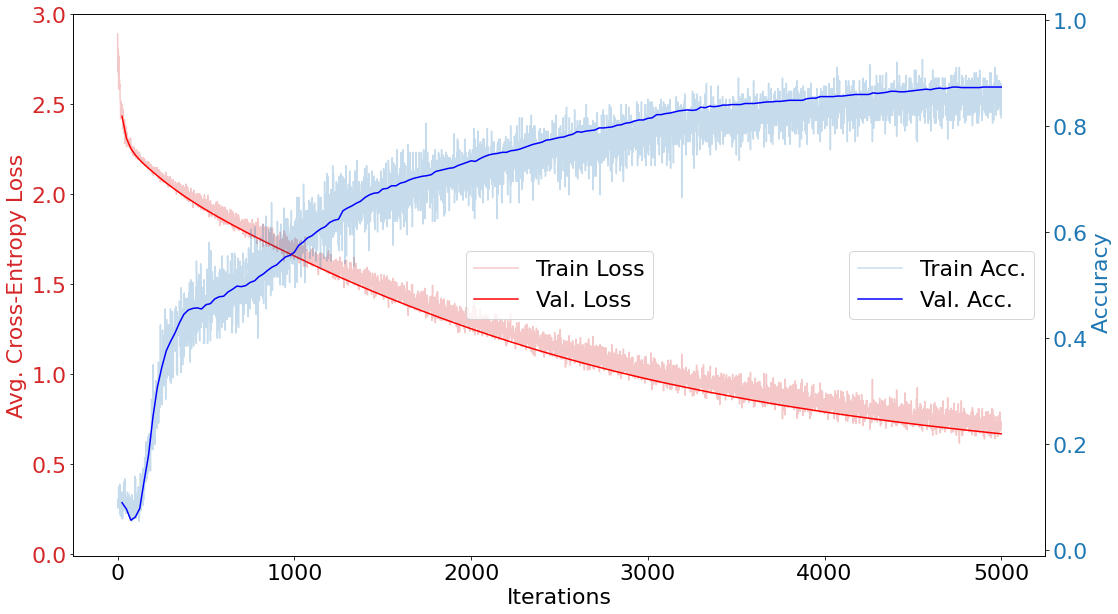
\includegraphics[width=0.7\textwidth]{figures/sigmoid.png}
\end{center}


\subsection{Analyzing Hyperparmeter Choices}
Neural networks have many hyperparameters. These range from architectural choices (\emph{How many layers? How wide should each layer be? What activation function should be used?}) to optimization parameters (\emph{What batch size for stochastic gradient descent? What step size (aka learning rate)? How many epochs should I train?}). This section has you modify many of these to examine their effect. The default parameters are below for easy reference.

\begin{center}
\begin{minipage}{0.9\textwidth}
\begin{lstlisting}[language=Python]
# GLOBAL PARAMETERS FOR STOCHASTIC GRADIENT DESCENT
np.random.seed(102)
step_size = 0.01
batch_size = 200
max_epochs = 200

# GLOBAL PARAMETERS FOR NETWORK ARCHITECTURE
number_of_layers = 2
width_of_layers = 16  # only matters if number of layers > 1
activation = "ReLU" if False else "Sigmoid" 
\end{lstlisting}
\end{minipage}
\end{center}


\xhdr{Optimization Parameters.} Optimization parameters in Stochastic Gradient Descent are very inter-related. Large batch sizes mean less noisy estimates of the gradient, so larger step sizes could be used. But larger batch sizes also mean fewer gradient updates per epoch, so we might need to increase the max epochs. Getting a good set of parameters that work well can be tricky and requires checking the validation set performance. Further, these ``good parameters'' will vary model-to-model.


\begin{taskbox}
\task{Q4 Learning Rate [2pts].}  The learning rate (or step size) in stochastic gradient descent controls how large of a step in the direction of the loss gradient we take our parameters at each iteration. The batch size determines how many data points we use to estimate the gradient. Modify the hyperparameters to run the following experiments:
\begin{enumerate}
    \item Step size of 0.0001 (leave default values for other hyperparameters)
    \item Step size of 5 (leave default values for other hyperparameters)
    \item Step size of 10 (leave default values for other hyperparameters)
\end{enumerate}
Include these plot in your report and answer the following questions:
\begin{enumerate}[a)]
\item Compare and contrast the learning curves with your curve using the default parameters. What do you observe in terms of smoothness, shape, and what performance they reach?
\item For (a), what would you expect to happen if the max epochs were increased?
\end{enumerate} 
\end{taskbox}



\xhdr{Activation Function and Depth.} As networks get deeper (or have more layers) they tend to become able to fit more complex functions (though this also may lead to overfitting). However, this also means the backpropagated gradient has many product terms before reaching lower levels -- resulting in the magnitude of the gradients being relatively small. This has the effect of making learning slower. Certain activation functions make this better or worse depending on the shape of their derivative. One popular choice is to use a Rectified Linear Unit or ReLU activation that computes:
%
\begin{equation}
    ReLU(x) = max(0,x)
\end{equation}
%
This is especially common in very deep networks. In the next question, we'll see why experimentally.

\begin{taskbox}
\task{Q5 ReLU's and Vanishing Gradients [3pts].} Modify the hyperparameters to run the following experiments:
\begin{enumerate}
    \item 5-layer with Sigmoid Activation (leave default values for other hyperparameters)
    \item 5-layer with Sigmoid Activation with 0.1 step size (leave default values for other hyperparameters)
    \item 5-layer with ReLU Activation (leave default values for other hyperparameters)
\end{enumerate}
Include these plot in your report and answer the following questions:
\begin{enumerate}[a)]
\item Compare and contrast the learning curves you observe and the curve for the default parameters in terms of smoothness, shape, and what performance they reach.  Do you notice any differences in the relationship between the train and validation curves in each plot? 
\item If you observed increasing the learning rate in (2) improves over (1), why might that be? 
\item If (3) outperformed (1), why might that be? Consider the derivative of the sigmoid and ReLU functions.
\end{enumerate}
\end{taskbox}



\subsection{Randomness in Training}
There is also a good deal of randomness in training a neural network with stochastic gradient descent -- network weights are randomly initialized and the batches are randomly ordered. This can make a non-trivial difference to outcomes. 

\begin{taskbox}
\task{Q6 Measuring Randomness [1pt].} Using the default hyperparameters, set the random seed to 5 different values and report the validation accuracies you observe after training. What impact does this randomness have on the certainty of your conclusions in the previous questions?
\end{taskbox}



\subsection{Make Your Kaggle Submission}

Great work getting here. In this section, you'll submit the predictions of your best model to the \href{https://www.kaggle.com/t/c4de5ee4c2ef45858c15e3183d24b2c0}{class-wide Kaggle competition}. You are free to make any modification to your neural network or the optimization procedure to improve performance; however, it must remain a feed-forward neural network! For example, you can change any of the optimization hyperparameters or add momentum / weight decay, vary the number of layers or width, add dropout or residual connections, etc.

\begin{taskbox}
\task{Q7 Kaggle Submission [8pt]}. Submit a set of predictions to Kaggle that outperforms the baseline on the public leaderboard. To make a valid submission, use the train set to train your neural network classifier and then apply it to the test instances in \texttt{mnist\_small\_test.csv} available from Kaggle's Data tab. Format your output as a two-column CSV as below:
\begin{verbatim}
id,digit
0,3
1,9
2,4
3,1
.
.
\end{verbatim}
where the id is just the row index in \texttt{mnist\_small\_test.csv}. You may submit up to 10 times a day. In your report, tell us what modifications you made for your final submission.
\end{taskbox}


\xhdr{Extra Credit and Bragging Rights [1.25pt Extra Credit].} The TA has made a submission to the leaderboard. Any submission outperforming the TA on the \emph{private} leaderboard at the end of the homework period will receive 1.25 extra credit points on this assignment. Further, the top 5 ranked submissions will ``win HW3'' and receive bragging rights. 






\section{Debriefing (required in your report)}
\begin{enumerate}
    \item Approximately how many hours did you spend on this assignment?
    \item Would you rate it as easy, moderate, or difficult?
    \item Did you work on it mostly alone or did you discuss the problems with others?
    \item How deeply do you feel you understand the material it covers (0\%–100\%)?
    \item Any other comments?
\end{enumerate}
\end{document}
